\Chapter{CONVOLUTIONAL NEURAL NETWORK WITH COMMENTS AND SOURCE CODE}\label{sec:Theme3}

% TOTAL = 15 pages

%	./train.py --enable_word_embeddings true --num_epochs 6 --dev_sample_percentage 0.01 --positive_train=$pos --negative_train=$neg
%	
%	Used for the 3-Folds
%
% ./word2vec -train ../../tokenized-concordia-no-comment.txt -output concordia-bin-64.bin -size 100 -window 5 -sample 1e-4 -negative 5 -hs 0 -binary 1 -cbow 1 -iter 3

\section{Convolutional Neural Network}

%1 page

Several machine learners were tested with TEDIOUS, using source code metrics as training features. Results were promising but the approach asked for a lot of preparation work: building the XML representation of the Java code, pattern matching between comments from the dataset and the original source code, extracting source code metrics, extracting warnings raised by automated static analysis tools and feature preprocessing. These preparation steps take time and require the knowledge of the whole process. Consequently, we wanted to experiment with a novel approach, easier and faster to set up. We decided to test a Convolutional Neural Network (CNN) with Natural Language Processing (NLP) directly on the Java source code of software projects.

The idea of using a CNN was inspired by a paper written by \citet{kim2014convolutional}. He used a CNN for sentence-level classification tasks and showed that you can achieve excellent performance results with little parameter calibration. To prove his point, he tested his model on a wide variety of benchmarks. \citet{dos2014deep} performed a similar work concerning sentiment analysis of short texts. More specifically, they analyzed Twitter messages and movie reviews, and tried to classify them as being of positive or negative sentiment. Our idea is similar to these studies, we plan to use a CNN to classify comments and/or methods using the source code directly instead of features, labeling them as technical debts or not.

Typically, convolutional neural networks were employed for image classification \citep{krizhevsky2012imagenet}, however, this type of neural network has also been used recently combined with NLP. To describe CNN in further details, we can think of a convolution as a window sliding across a whole matrix. This window is in fact acting like a filter. For images, this matrix contains pixels, for words and sentences, it contains word vectors (word embeddings). In image classification, filters slide over local batches, in NLP, they slide over entire rows since a row is typically a single word embedded into a row matrix of the size of the embedding dimension. To implement a CNN, you just have to add several layers of these convolutions, where each of these layers have a specific task and acts as different filters. CNNs are very fast and efficient to provide good representations of datasets even with a partial vocabulary. Figure \ref{fig:example} presents an example of a CNN architecture.

\begin{figure}[t]
	\centering
	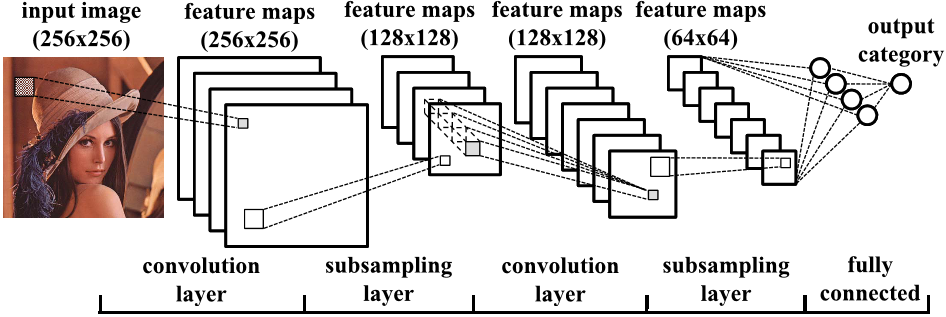
\includegraphics[width=\linewidth]{figs/CNN-example.png}
	\caption{An example of a convolutional neural network \citep{Cong2014MinimizingCI}.}
	\label{fig:example}
	\vspace{-4mm}
\end{figure}

The main purpose of this thesis was to explain, test and analyze TEDIOUS, our machine learning approach using source code features. The next sections will describe the other approach using a CNN, but less in depth than for TEDIOUS since it is still at its preliminary stages. However, we still judged interesting to present the initial results of this alternative method. Since some steps from Chapter 3 are replicated in our CNN approach, they will be reviewed summarily.

\section{The Approach}

%1 page

This section will describe the steps followed to design this new approach, a convolutional neural network combined with natural language processing to identify technical debts to self-admit. Like TEDIOUS, this approach works at method-level since it is the granularity at which we are most likely to detect TD \citep{PotdarS14}. In other terms, this approach is able to detect if a technical debt is contained in a method or not.
 
\begin{figure}[t]
	\centering
	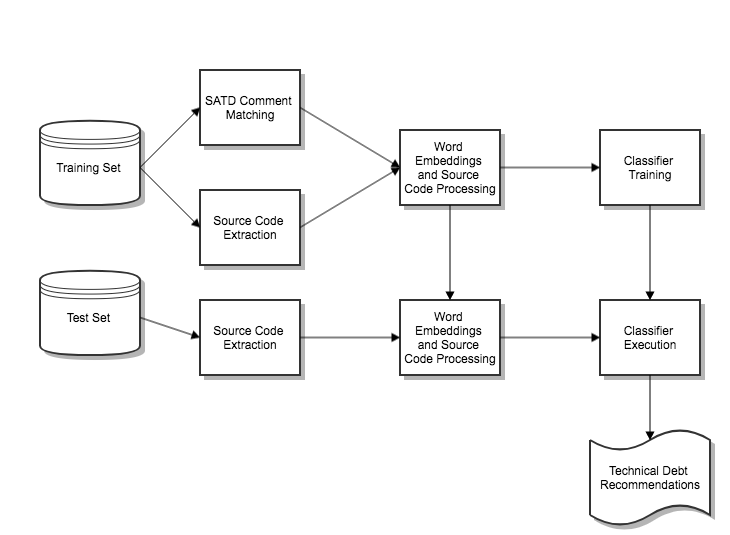
\includegraphics[width=\linewidth]{figs/CNN.png}
	\caption{Proposed approach for recommending SATD with a CNN.}
	\label{fig:CNN}
	\vspace{-4mm}
\end{figure}

The implementation of the CNN is based on the work of \citet{kim2014convolutional} and Britz (2015). As shown in Figure \ref{fig:CNN}, two datasets are required to build our model: the training and test set. The training set contains labeled data, which is source code where SATD are known. The test set contains unlabeled data, which can be any source code where we want to recommend where technical debts should be admitted.

For the training set, various combinations of source code and comments, labeled as containing a SATD or not, are extracted: source code comments only, source code with comments, source code without comments and source code partially with comments. It is essential to have this classification because the CNN is based on supervised learning. Pattern matching using comments from the dataset of \citet{maldonado17} is employed to classify methods and comments.

Once all the source code is extracted and classified, it still has to be preprocessed. The source code is tokenized, the purpose being to demarcate and transform the source code into a string of word tokens. The comments specifically are cleaned up to remove extra spaces, non-ASCI characters, upper-case letters, etc. Once the source code is preprocessed, word embeddings is performed, which means strings of tokens are transformed into vectors of numerical values using word2vec tool. With the source code preprocessed and the oracle built, the model can be trained with the CNN.

But before, in parallel, the test set is prepared. The same combinations of source code and comments are extracted, but SATD matching is not required because the data is unlabeled and we want to predict the presence of technical debts. The same preprocessing and word embeddings are applied on the test dataset. With the previously trained model and the test set, predictions can be made in order to recommend when to self-admit technical debts.

An overview of the process was described in this section, but more details will be shared in the next ones. We will discuss the source code and its nature, how we identified the SATD, how we performed word embeddings and the process to train and apply the models generated by the CNN.

\subsection{Source Code}

% 1 page

The main difference between TEDIOUS and this new approach is the nature of the training features. For TEDIOUS, source code metrics and warnings were used. For the CNN, we use the source code itself, transformed into word vectors. The same process as before was performed to extract the source code, where an XML representation of the Java source code was generated using the srcML tool \citep{Collard2013}. To build the oracle, SATD comments from the dataset of \citet{MaldonadoNLP} were linked to their respective methods in the studied projects in order to classify them as containing a technical debt or not. The same rules were followed, as explained in Section 3.1.1 Features for TEDIOUS. Once the XML representation is obtained, the different dataset combinations can be generated.

The first feature combination is \textit{source code comments only}. They are extracted from the dataset of comments provided by \citet{maldonado17}. Comments can be encountered under different forms: single line, multiple lines or block. Single line comments are comments written on a single line of code. They use the \textsc{(// ...)} commenting method. Multiple line comments are several single line comments grouped together. Block comments are comments written over several lines of code but that are considered as a single entity. They use the \textsc{(/* ... */)} commenting method.

Like TEDIOUS, it is important to specify that solely design debts were retained. We decided to use only this type of SATD-method in order to have the same basis of comparison between TEDIOUS and our CNN. However, by doing so, we maintain the unbalance of the dataset which could be diminished by adding more positive examples in the form of other types of SATD-methods.

The second combination is \textit{source code with comments} where the complete XML representation of the source code is used. The third combination is \textit{source code without comments} where the XML representation is parsed to remove comments. The fourth combination is \textit{source code partially with comments}, which means only comments related to SATD are removed. The reason behind this removal is to be sure to avoid the CNN model being a self-prophecy. For these three datasets, only design TDs are retained, to be in line with the dataset used by TEDIOUS. The details of the process behind the extraction of each combination will be explained in the Source Code Preprocessing section.

\subsection{Identification of Self-Admitted Technical Debt}

% 0.5 page

Like TEDIOUS, the purpose of this approach is not to propose a new way to detect SATD using information from comments. However, will still need a classified dataset of SATD comments in order to train our CNN model. We used the dataset of \citet{maldonado17}, which contains a classification of 10 open source projects, where comments are tagged as relating to a technical debt or not. Various types of TDs are considered, depending on the source code combination. The dataset reports SATD at file-level instead of method-level, consequently, some preprocessing had to be performed using pattern matching to tag SATD comments to their related methods.

\subsection{Source Code Preprocessing and Word Embeddings}

% 1 page

The source code is extracted in a XML format, which is not quite compatible for the machine learner to train on. To make it compatible, XML files have to be tokenized. Instead of using standard coding lexicon (conditional statements, variable types and names, parameters declaration) and separators (brackets, parentheses, spaces) directly in our dataset, demarcations are added (\textit{i.e. begin\_type, end\_type}) to transform the structure into series of word tokens. For comments, strings are normalized: extra spaces are removed, upper cases are transformed to lower cases, non-ASCI are removed as well as new lines. Also, if a comment is matched with a SATD pattern, it will be delimited with the following tokens: \textsc{comment\_begin\_satd} and \textsc{comment\_end\_satd}. 

This step is essential to build the oracle and the dataset partially with comments. By explicitly defining comments tagged as SATD in this format, it is easy to parse the tokenized dataset in order to remove them. Comments are linked to their respective method, so a method linked to a SATD comment will also be tagged as SATD. By tokenizing the source code, it is also easier to remove the comments entirely, if necessary. Transforming the source code into tokens also acts as a normalization process, which will make the word embedding process more efficient. Here is a code snippet of what the source code looks like before and after the tokenization.

\newpage

\begin{mdframed}
	\begin{lstlisting}
	/**
	* Add a nested task.
	* <p>
	* @param nestedTask  Nested task to execute
	* <p>
	*/
	public void addTask(Task nestedTask) {
	nestedTasks.addElement(nestedTask);
	}
	\end{lstlisting}
\end{mdframed}

\begin{mdframed}
	\begin{center}
		 begin\_comment add a nested task p param nested task nested task to execute p end\_comment  begin\_type  begin\_specifier  end\_specifier  begin\_name void  end\_name  end\_type  begin\_name add task  end\_name  begin\_parameter\_list  begin\_param  begin\_decl  begin\_type  begin\_name task  end\_name  end\_type  begin\_name nested task  end\_name  end\_decl  end\_param  end\_parameter\_list  begin\_block  begin\_expr\_stmt  begin\_expr  begin\_call  begin\_name  begin\_name nested tasks  end\_name  begin\_operator DOT  end\_operator  begin\_name add element  end\_name  end\_name  begin\_argument\_list  begin\_argument  begin\_expr  begin\_name nested task  end\_name  end\_expr  end\_argument  end\_argument\_list  end\_call  end\_expr  end\_expr\_stmt  end\_block 
	\end{center}
\end{mdframed}

Word embeddings is the process of transforming words and phrases from the dataset into vectors of real number. Word2vec models were used to generate word embeddings. The vector dimension we used is 150 because we tried to have a balance between a proper representation of words and processing time. A new word embedding was generated for each source code combination since they are all different in some ways.

Finally, the methods extracted are all tagged as positive or negative examples. In order for the CNN to be trained and tested, these methods have to be divided in 4 standard files: \textsc{positive-train}, \textsc{negative-train}, \textsc{positive-test} and \textsc{negative-test}. Each fold of the cross validation contains these 4 files, consequently, for a 10-fold cross validation, 40 files are required. Instead of using an additional feature to classify each method in a single file, the files act as classifier entities. Here is a detailed definition of each file, considering a 10-fold cross validation:

\newpage

\begin{itemize}
	\item \textit{Positive-Train}: Training set containing SATD methods (90\% of all positive examples)
	\item \textit{Negative-Train}: Training set containing non-SATD methods (90\% of all negative examples)
	\item \textit{Positive-Test}: Testing set containing SATD methods (10\% of all positive examples)
	\item \textit{Negative-Test}: Testing set containing non-SATD methods (10\% of all negative examples)
\end{itemize}

\begin{figure}
	\centering
	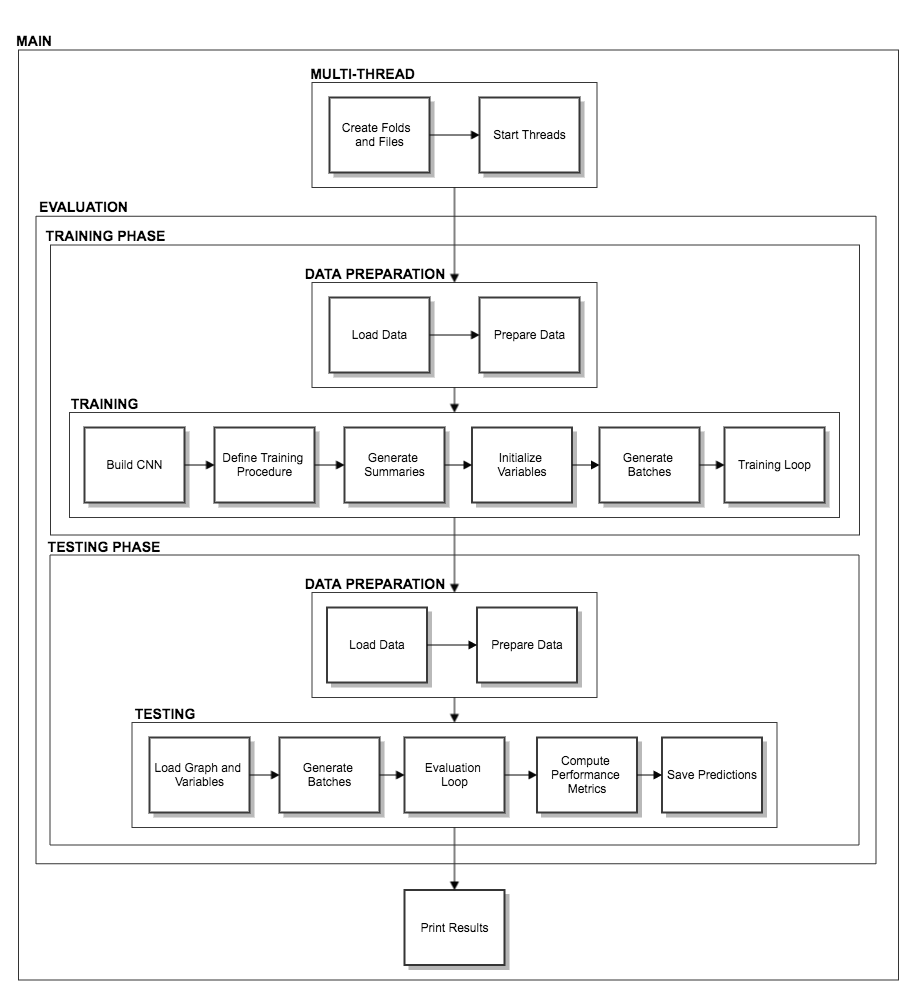
\includegraphics[width=\linewidth]{figs/CNNProcess.png}
	\caption{Process for building and applying a CNN.}
	\label{fig:CNNProcess}
	\vspace{-4mm}
\end{figure}

\subsection{Building and Applying CNN}

% 2 page

So far, we extracted source code from various projects, with or without comments, we identified SATD methods, we preprocessed the dataset and performed a word embedding. The only step remaining is building and applying the convolutional neural network. Four datasets are required, as described in the previous section: two sets for training, one containing SATD methods and the other not, and two sets for testing, one of positive and the other of negative examples. The sets contain the tokenized source code of the 9 studied projects, divided between them.

Figure \ref{fig:CNNProcess} provides an overview of the CNN process. To increase the training speed and to benefit as much as possible from the processing power available, several threads are created. One thread is started for each fold, feeding it with a pair of previously generated training files. Up to five threads can be processed at the same time. The next actions are all performed simultaneously on each thread, until we have models trained for all folds. 

The evaluation process consists of two main phases: the training and the testing phase. In the former, some data preparation is required: load the two training sets, build the vocabulary, shuffle the datasets, and split the dataset in a training and development set. The development set is used to tune parameters of the CNN and to prevent it from over-fitting during the training process. Afterwards, the CNN is built using user-defined parameters and default values. In our case, mainly the default configuration is considered. Here is a list of the standard hyper-parameters used with their values.

\newpage

% https://github.com/dennybritz/cnn-text-classification-tf
\begin{itemize}
\item \textit{ALLOW\_SOFT\_PLACEMENT = True}, to find out which devices your operations and tensors are assigned to.
\item \textit{BATCH\_SIZE = 32}, to define the batch size for each training loop.
\item \textit{CHECKPOINT\_EVERY = 100}, to save the model after this many steps.
\item \textit{DEV\_SAMPLE\_PERCENTAGE = 0.01}, to define the percentage of the training data to use for validation.
\item \textit{DROPOUT\_KEEP\_PROB = 0.5}, to define the dropout keep probability. \textit{Dropout} is a technique to prevent neural networks from overfitting \citep{srivastava2014dropout}. 
\item \textit{EMBEDDING\_DIM = 150}, to define the dimension size of the word embeddings.
\item \textit{ENABLE\_WORD\_EMBEDDINGS = True}, to enable word embeddings.
\item \textit{EVALUATE\_EVERY = 100}, to evaluate the model on the development set after this many steps.
\item \textit{FILTER\_SIZES = 3,4,5}, to define the filter sizes.
\item \textit{L2\_REG\_LAMBDA = 0.0}, to define the L2 regularization lambda.
\item \textit{LOG\_DEVICE\_PLACEMENT = False}, to enable log placement of operations on devices.
\item \textit{NUM\_CHECKPOINTS = 5}, to define the number of checkpoints to store.
\item \textit{NUM\_EPOCHS = 6}, to define the number of training epochs.
\item \textit{NUM\_FILTERS = 128}, to define the number of filters per filter size.
\end{itemize}

The training procedure is defined before executing it and summaries are generated during the process for: loss, accuracy, train, development and model. Then, variables are initialized, such as embedding vectors, and training batches are generated. Finally, a training loop is executed where training and evaluation steps are repeated. The trained model is saved multiple times during the loop and the last one is used for the testing. 

We can start the testing phase once the training is finished. Data preparation is also required for this step: load the two testing sets and map them into the vocabulary. Afterwards, the meta graph and the variables from the model previously trained are loaded. Testing batches are generated and tensors we want to evaluate are created. Then, we can start the testing loop where predictions are made. Once done, performance metrics can be computed: accuracy, recall, precision, specificity and $F_1$. These metrics are saved in a different file from the file containing predictions made on each method. The final step consists of combining performance metrics of all models for further analysis.

\section{Study Definition}

% 0.5 page

The goal of this new approach is to assess the prediction performance of a convolutional neural network in recommending technical debts to self-admit. The focus is the same as for TEDIOUS, enhancing the source code quality by keeping track of TDs. The perspective is to be able to suggest to developers, more accurately than with TEDIOUS, when to admit technical debts. We aim to address four research questions:

\begin{itemize}
	\item \textbf{RQ1}: How does a CNN work for recommending SATD with source code comments only?
	\item \textbf{RQ2}: How does a CNN work for recommending SATD with source code  with comments?
	\item \textbf{RQ3}: How does a CNN work for recommending SATD with source code without comments?
	\item \textbf{RQ4}: How does a CNN work for recommending SATD with source code partially with comments?
\end{itemize}

\subsection{Dataset}

% 1.5 page

	\begin{table*}[t]
		\caption{Characteristics of the studied projects.}
		\label{tab:projectsCNN}
		\centering
		\begin{adjustbox}{center}
			\begin{tabular}{l r | r r | r | r}
				\hline
				\multirow{2}{*}{Project} & \multirow{2}{*}{Release} &\multicolumn{2}{c|}{Number of} 
				&\multicolumn{1}{c|}{Number of Design SATD} & \% of Methods\\
				&&  Methods& Comments & $\in$ Methods & with design SATD\\
				\hline
				Ant&1.7.0 & 12025 & 14406& 60& 0.5\% \\
				ArgoUML&0.34& 16277 & 23113 & 1041& 6.4\%\\
				Columba&1.4& 8554 & 12355 &119 & 1.4\%  \\
				Hibernate&3.3.2 GA & 19285 & 10657 &313 & 1.6\%\\
				jEdit & 4.2 & 5390 & 11880 &97 & 1.8\% \\
				jFreeChart&1.0.19 & 11252 & 17091& 182& 1.6\%\\
				jMeter&2.1& 9825 & 14681 &222 & 2.3\%  \\
				jRuby&1.4.0 & 15385 & 9084 &389 &2.5\%\\
				Squirrel&3.0.3 & 18328 & 17469 &106 & 0.6\%\\
				\hline
			\end{tabular}
		\end{adjustbox}
		\vspace{-4mm}
	\end{table*}

To evaluate this new approach, the same dataset was used as in TEDIOUS \citep{maldonado17}. Methods are already classified as SATD or not, and Table \ref{tab:projectsCNN} summarizes the characteristics of all studied projects, where various information describe the content and nature of each project. A similar table was shown previously (Table \ref{tab:projects}) but some modifications were made for the CNN.

Firstly, there are some discrepancies between the results we obtained when analyzing the studies and what \citet{maldonado17} obtained. However, this does not really represent an issue since many of those differences concern classes while our CNN approach is method-level based, like TEDIOUS. This aspect is also important since we clearly see the prevalence of method-related rather than class-related SATD (see Table \ref{tab:projects}). Out of all methods in a project, only a very small amount contains technical debts, making the dataset highly unbalanced. As we will discuss in the analysis of results, the lower the number of technical debts in a system, the lower the prediction performance. Additionally, since the dataset from \citet{maldonado17} classified classes instead of methods, we performed pattern matching between known SATD comments and comments attached to methods in the dataset.

As for the disparities between Table \ref{tab:projects} and Table \ref{tab:projectsCNN}, they can be explained by the philosophy behind the matching of SATD comments with methods. For Table \ref{tab:projects}, the number and percentage of methods containing a design SATD is based on the number of times a comment is tagged as SATD. This means that a method could contain three different comments referring to a design technical debt or a comment could be matched with several SATD comment patterns. Therefore, a method could be tagged several times as one containing a technical debt.

For Table \ref{tab:projectsCNN}, the number and percentage of methods containing a design technical debt represent the absolute number of methods containing a TD. This means that even though a method contains several SATD comments or is tagged several times as a problematic method, it will only be counted once. Consequently, the number of methods containing a TD is exactly the same number of methods that the CNN is being trained and tested on. To observe this disparity, we see that the number of methods with a design technical debt in jFreeChart is 1881 in Table \ref{tab:projects} and 182 in Table \ref{tab:projectsCNN}. Therefore, we will base the analysis of results of the CNN on Table \ref{tab:projectsCNN}.

\subsection{Analysis Method}

% 2 pages

\begin{table}[t]
	\caption{Within-project prediction: results of CNN for each system using source code comments only}
	\label{tab:commentsonly}
	\centering\tiny
	\resizebox{\linewidth}{!}{
		
		\begin{tabular}{lrrrr}
			%\hline
			\multicolumn{5}{c}{ \textbf{Source Code Comments Only}}\\
			\hline
			\textbf{System} & \textbf{Pr} & \textbf{Rc }&\textbf{F$_{1}$} &\textbf{Acc}\\
			\hline
			Ant & 66.67 & 12.00 & 20.34 & 99.49\\
			ArgoUML & 85.80 & 73.09 & 78.93 & 97.08\\
			Columba & 89.55 & 56.60 & 69.36 & 98.90\\
			Hibernate & 78.08 & 59.58 & 67.59 & 96.85\\
			jEdit & 100.00 & 3.33 & 6.45 & 97.76\\
			jFreeChart & 95.39 & 86.31 & 90.63 & 99.73\\
			jMeter & 78.57 & 61.42 & 68.95 & 98.27\\
			jRuby & 89.11 & 63.69 & 74.29 & 95.82\\
			Squirrel & 82.76 & 26.67 & 40.34 & 99.16\\
			\textbf{Total} & \textbf{85.49} & \textbf{62.61} & \textbf{72.28} & \textbf{98.38}\\
			\hline
		\end{tabular}
	}
	\vspace{-3mm}
\end{table}

For \textbf{RQ1}, we want to know how a convolutional neural network with \emph{source code comments only} work for recommending SATD within project. We also want to compare the results with the within project predictions of TEDIOUS. A 10-fold cross validation was performed on each project, like for TEDIOUS, and the performance values are averaged over the 10 iterations. The same process is followed for \textbf{RQ2}, \textbf{RQ3} and \textbf{RQ4}.

Standard performance metrics on the SATD category were computed to evaluate our automated classification approach: precision, recall, $F_1$ score and accuracy. Precision is the percentage of relevant instances of methods predicted as SATD among all retrieved instances. Recall is the percentage of relevant instances of SATD methods that have been retrieved over all relevant instances. $F_1$ score is the harmonic mean between precision and recall. Accuracy is the total number of methods correctly predicted, whether it is SATD-related or not, among all analyzed methods. 

%% VOIR SI ON PEUT EVALUER ROC OU AUX
%%  I am wondering if there is any way we intercept the score/probability before the final class assigmnement this could led to evaluation roc/auc …

%Unfortunately, metrics such as MCC, ROC and importance of features were not computed for this approach. However, we still have enough information to evaluate and compare each approach. The downside is that it will be more difficult to take into account the effect of chance on predictions. 
Overall, what we look for in a good classifier is a balance between precision and recall while aiming for the highest $F_1$ score. We want to detect as many technical debts as possible while being correct in our predictions.

\section{Study Results}

This section reports the results obtained using various combinations of source code. Performance metrics are presented in tables and further analysis is provided textually, discussing the metrics and comparing them with TEDIOUS.

%% DO CROSS PROJECT
%%   should we/can we do it cross-project say one project out? should be easy …

\subsection{Source Code Comments Only}

%1.5 pages 

Table \ref{tab:commentsonly} reports the within project performance results of a 10-fold cross validation on each system using our convolutional neural network and source code comments only. We computed the average for the 10 folds of each system and for the complete dataset. Since we already had the comments preprocessed for TEDIOUS, this dataset was a good start to test our CNN approach.

Three systems perform worse than the others, namely \textsc{Ant}, \textsc{jEdit} and \textsc{Squirrel}, especially for the recall. We can visualize this fact in Figure \ref{fig:comments-only-pred}. We face the same problem as in TEDIOUS, where the very low percentage and absolute number of SATD methods (\textsc{Ant} has 60 instances for 0.5\% of methods, \textsc{jEdit} has 97 instances for 1.8\% of methods and \textsc{Squirrel} has 106 instances for 0.6\% of methods) in some systems directly affects the performance of the CNN. \textsc{Ant} obtains a precision of 66.67\%, recall of 12.67\% and $F_1$ score of 20.34\%. \textsc{jEdit} is worse, it has a precision of 100.00\% but a recall of 3.33\% and a $F_1$ score of 6.45\%. \textsc{Squirrel} obtains a precision of 82.76\% but a recall of only 26.67\%. However, if we compare with results from TEDIOUS, we notice a significant improvement in precision while maintaining a similar or worse recall for these two systems.

\begin{figure}[h]
	\centering
	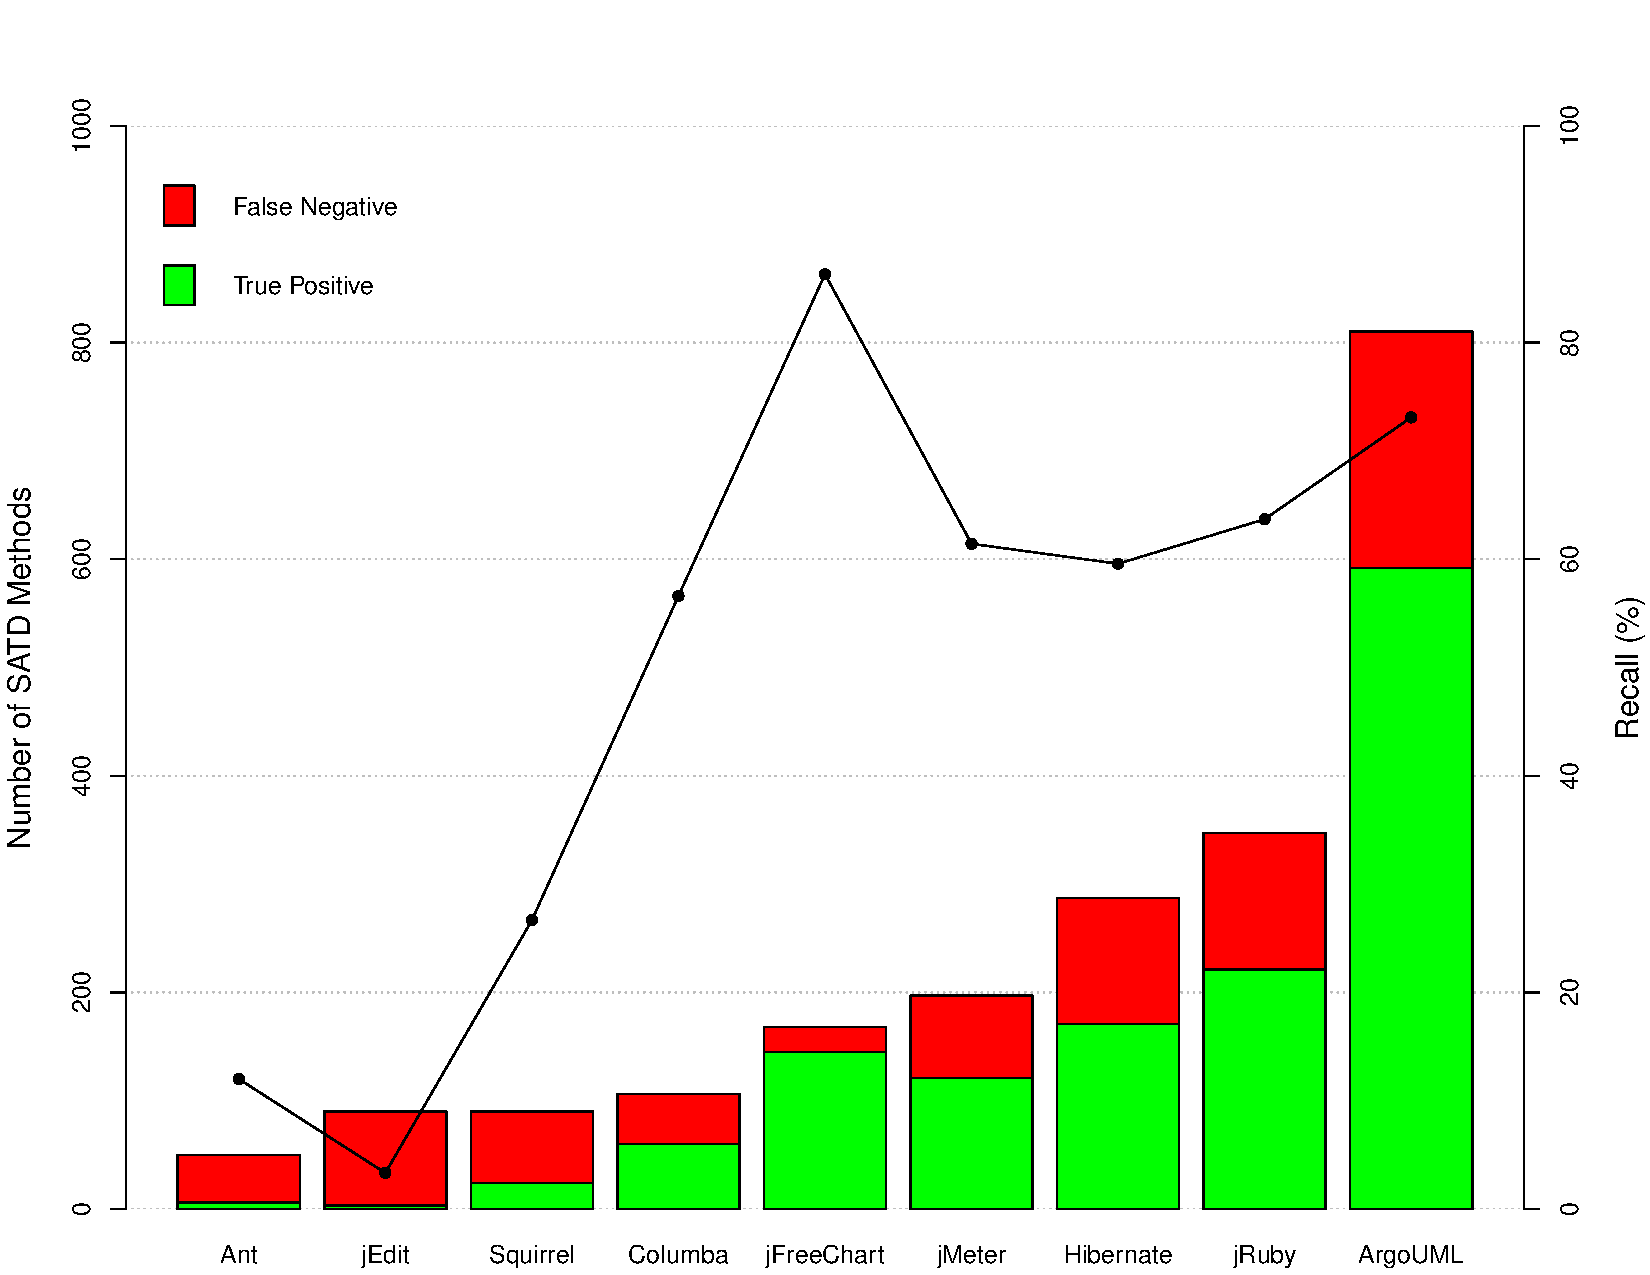
\includegraphics[scale=0.5]{figs/comment-only-pred.pdf}
	\caption{Comments only predictions.}
	\label{fig:comments-only-pred}
	\vspace{-4mm}
\end{figure}

\begin{table}[t]
	\caption{Within-project prediction: results of CNN for each system using source code with comments}
	\label{tab:comments}
	\centering\tiny
	\resizebox{\linewidth}{!}{
		
		\begin{tabular}{lrrrr}
			%\hline
			\multicolumn{5}{c}{ \textbf{Source Code With Comments}}\\
			\hline
			\textbf{System} & \textbf{Pr} & \textbf{Rc }&\textbf{F$_{1}$} &\textbf{Acc}\\
			\hline
			Ant & 66.67 & 12.00 & 20.34 & 99.61 \\
			ArgoUML & 82.64 & 86.42 & 84.49 & 96.99 \\
			Columba & 88.00 & 62.27 & 72.93 & 99.43 \\
			Hibernate & 83.73 & 73.52 & 78.29 & 98.80 \\
			jEdit & 83.33 & 5.55 & 10.42 & 98.40 \\
			jFreeChart & 94.34 & 89.29 & 91.74 & 99.53 \\
			jMeter & 77.84 & 65.99 & 71.43 & 98.94 \\
			jRuby & 85.88 & 85.88 & 85.88 & 98.75 \\
			Squirrel & 82.05 & 35.56 & 49.61 & 99.29 \\
			\textbf{Total} & \textbf{84.06} & \textbf{74.50} & \textbf{78.99} & \textbf{98.89}\\
			\hline
		\end{tabular}
	}
	\vspace{-3mm}
\end{table}

As for the other systems, the precision is $> 78\%$, the recall is $> 56\%$ and the $F_1$ $> 67\%$. Like TEDIOUS, the best results were obtained with \textsc{jFreeChart} (precision 95.39\%, recall 86.31\% and $F_1$ 90.63\%). Other projects such as \textsc{ArgoUML} or \textsc{jRuby} also provided good performance values. It is interesting to notice that \textsc{ArgoUML} and \textsc{jRuby} have respectively the two highest number of methods containing a design technical debt, with 1041 and 389 instances. \textsc{jFreeChart} does not have the most technical debts but still obtains the best recall, as shown in Figure \ref{fig:comments-only-pred}.

On first look, it seems that the CNN approach using source code is an improvement over TEDIOUS using source code features. The total average precision, recall and $F_1$ score is almost as good as the best system using TEDIOUS for within project validation. Further testing is required to provide a better understanding of the CNN's performance, which will be accomplished in the next sections.


% \Desktop\CNN-results.csv
% \noiseux1523\cnn-text-classification-tf-w2v 
%		dans \encoded-comment-files pour le data
%		dans \run-all.sh pour le process

\subsection{Source Code With Comments}

%1.5 pages

Using source code comments only is an interesting first step to train a convolutional neural network to predict technical debts, especially if we aim at addressing the issue of self-admitted technical debts. However, it would also be interesting to see how well a CNN can perform using the entirety of a project's source code, code and comments included. We experimented with such a dataset and obtained the results reported in Table \ref{tab:comments} for a within project 10-fold cross validation.

Again, as shown in Figure \ref{fig:all-comments-pred}, the worst results were obtained for \textsc{Ant}, \textsc{jEdit} and \textsc{Squirrel}. Compared to source code comments only, \textsc{Ant} obtained the same precision (66.67\%) and $F_1$ (20.34\%) but worsened its recall by $- 0.67\%$. \textsc{jEdit} worsened its precision by $- 16.67\%$ and improved its recall by $+ 2.22\%$. \textsc{Squirrel} obtained a similar precision  but increased its recall. We notice that the unbalance of the dataset is still an issue for the CNN but these results are still better than what we obtained with TEDIOUS.

\begin{figure}[h]
	\centering
	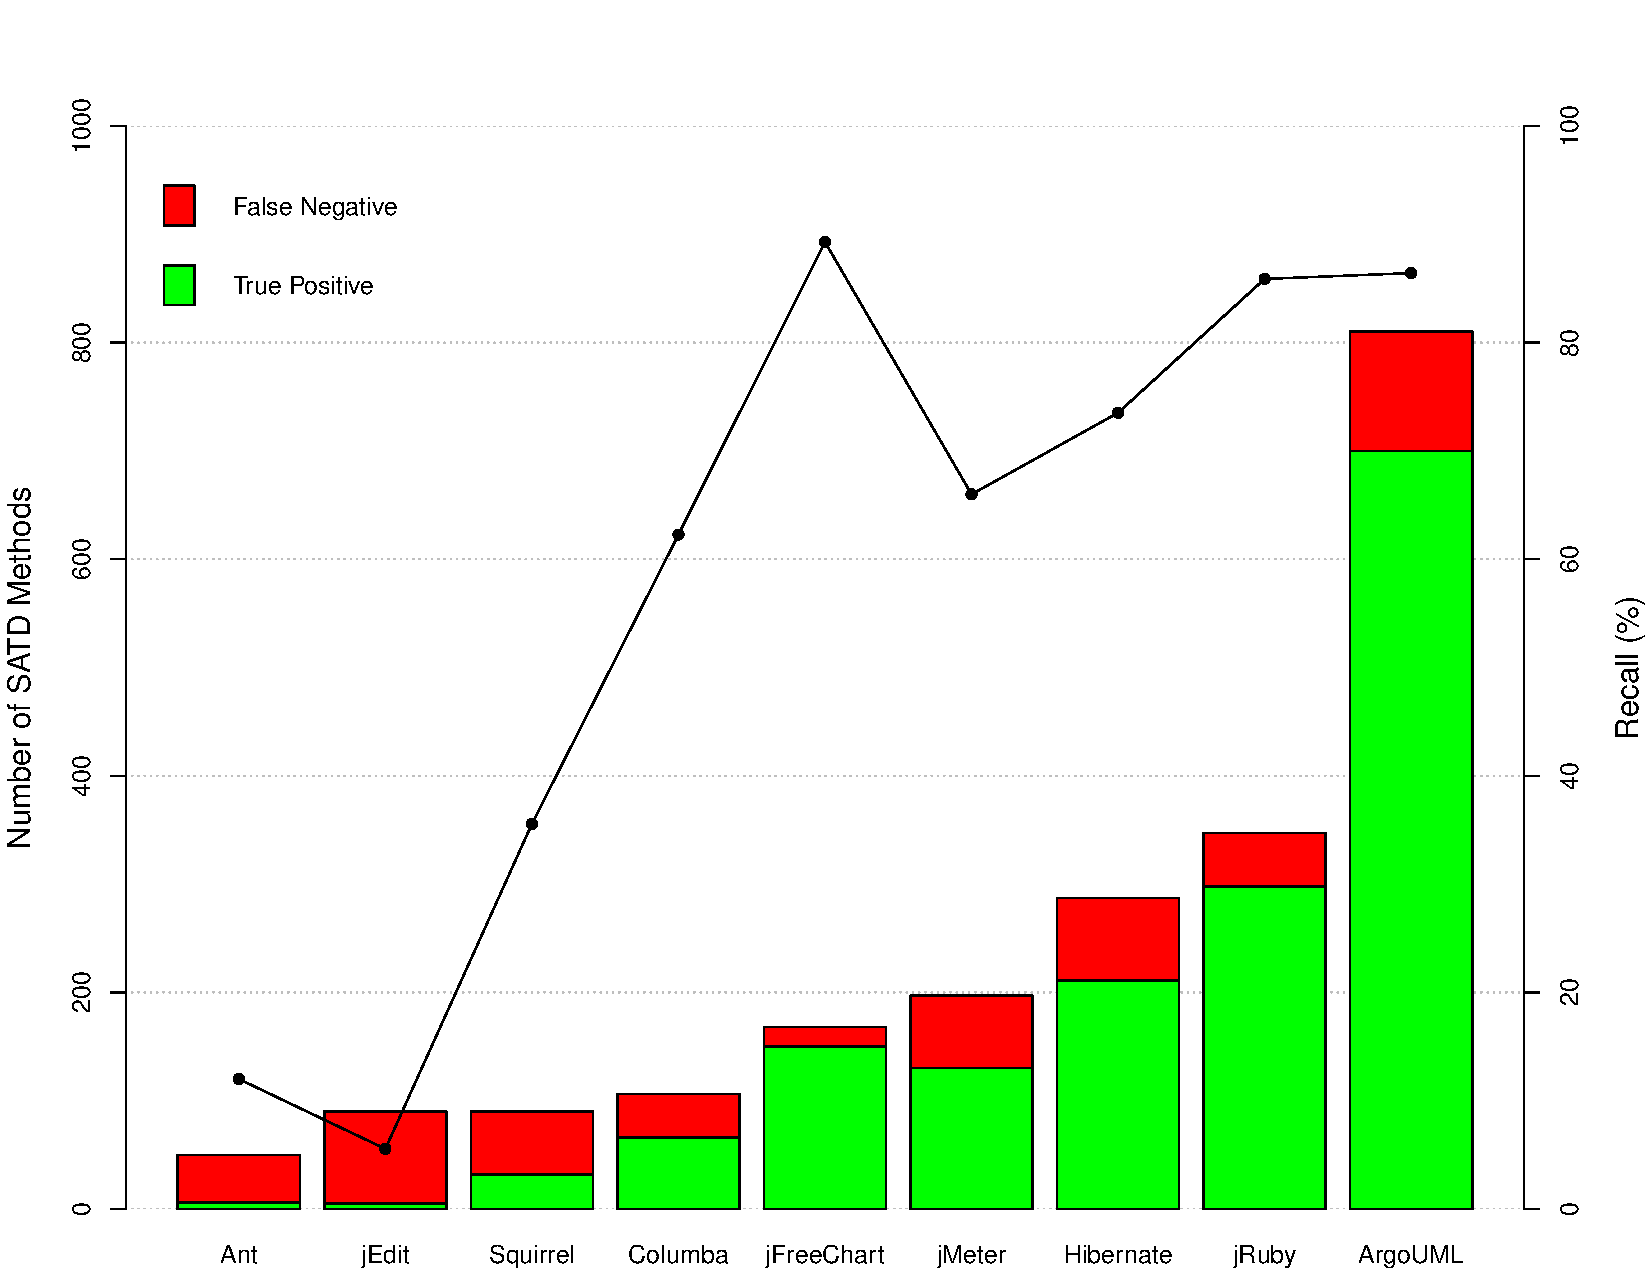
\includegraphics[scale=0.5]{figs/all-comments-pred.pdf}
	\caption{Comments and methods predictions.}
	\label{fig:all-comments-pred}
	\vspace{-4mm}
\end{figure}

As for the other systems, the precision varies between $[77.84\%-94.34\%]$, the recall between $[62.27\%-89.29\%]$ and the $F_1$ score between $[71.43\%-91.74\%]$. Precision is slightly worst but recall is improved compared to the source code comments only dataset. The best results were obtained with \textsc{jFreeChart} (precision $94.34\%$, recall $89.29\%$ and $F_1$ score $91.74\%$), followed closely by \textsc{ArgoUML} and \textsc{jRuby}, like in TEDIOUS and the previous dataset. This is not surprising since the only difference between the two datasets is the amount of information provided, where methods' source code is added in this current configuration.

\begin{table}[t]
	\caption{Within-project prediction: results of CNN for each system using source code without comments}
	\label{tab:withoutcomments}
	\centering\tiny
	\resizebox{\linewidth}{!}{
		
		\begin{tabular}{lrrrr}
			%\hline
			\multicolumn{5}{c}{ \textbf{Source Code Without Comments}}\\
			\hline
			\textbf{System} & \textbf{Pr} & \textbf{Rc }&\textbf{F$_{1}$} &\textbf{Acc}\\
			\hline
			Ant & 0 & 0 & 0 & 99.52 \\
			ArgoUML & 78.31 & 32.10 & 45.53 & 92.72 \\
			Columba & 55.00 & 10.38 & 17.46 & 98.78 \\
			Hibernate & 49.01 & 25.78 & 33.79 & 97.04 \\
			jEdit & 37.50 & 3.33 & 6.12 & 98.29 \\
			jFreeChart & 75.29 & 38.10 & 50.59 & 97.81 \\
			jMeter & 31.25 & 5.08 & 8.73 & 97.87 \\
			jRuby & 75.00 & 43.23 & 54.84 & 96.86 \\
			Squirrel & 33.33 & 2.22 & 4.17 & 99.00 \\
			\textbf{Total} & \textbf{68.17} & \textbf{26.76} & \textbf{38.43} & \textbf{97.61}\\
			\hline
		\end{tabular}
	}
	\vspace{-3mm}
\end{table}

If we look at the average total performance values, there are small differences compared to the source code comments only dataset: precision $- 1.43\%$, recall $+ 11.89\%$ and $F_1$ $+ 6.71\%$. Consequently, using the whole source code is also an improvement compared to TEDIOUS as well as source code comments only. Adding more information enhanced the prediction power of our model, especially for the recall rate. However, precision was affected by the introduction of more training material, which could have caused noise in the dataset. If we value more the time required to train models, using comments only would be preferred since it is ten times faster than source code with comments. If we value more the performance, then source code with comments is the best configuration to use.

We just tested the best case scenario where we have as much information as possible to train on, however, we also want to know how well a CNN can perform on a less than ideal software project.

% \Desktop\stats-baseline-with comments.csv
% dans \yes-and-no pour le data
% dans \run-all.v2.sh pour le process

\subsection{Source Code Without Comments}

%1.5 pages

We trained our convolutional neural network on source code comments only and on source code with comments. We obtained promising results, but we want to know how well our machine learner can work with less training features. We generated another dataset, this time only containing the source code of the studied projects, eliminating the comments. We built such a dataset to replicate the worst case where a software project is lacking comments and to remove SATD comments related to their respective methods. Table \ref{tab:withoutcomments} reports the performance results for each system using a 10-fold cross validation and source code without comments as the training set.

\begin{figure}[h]
	\centering
	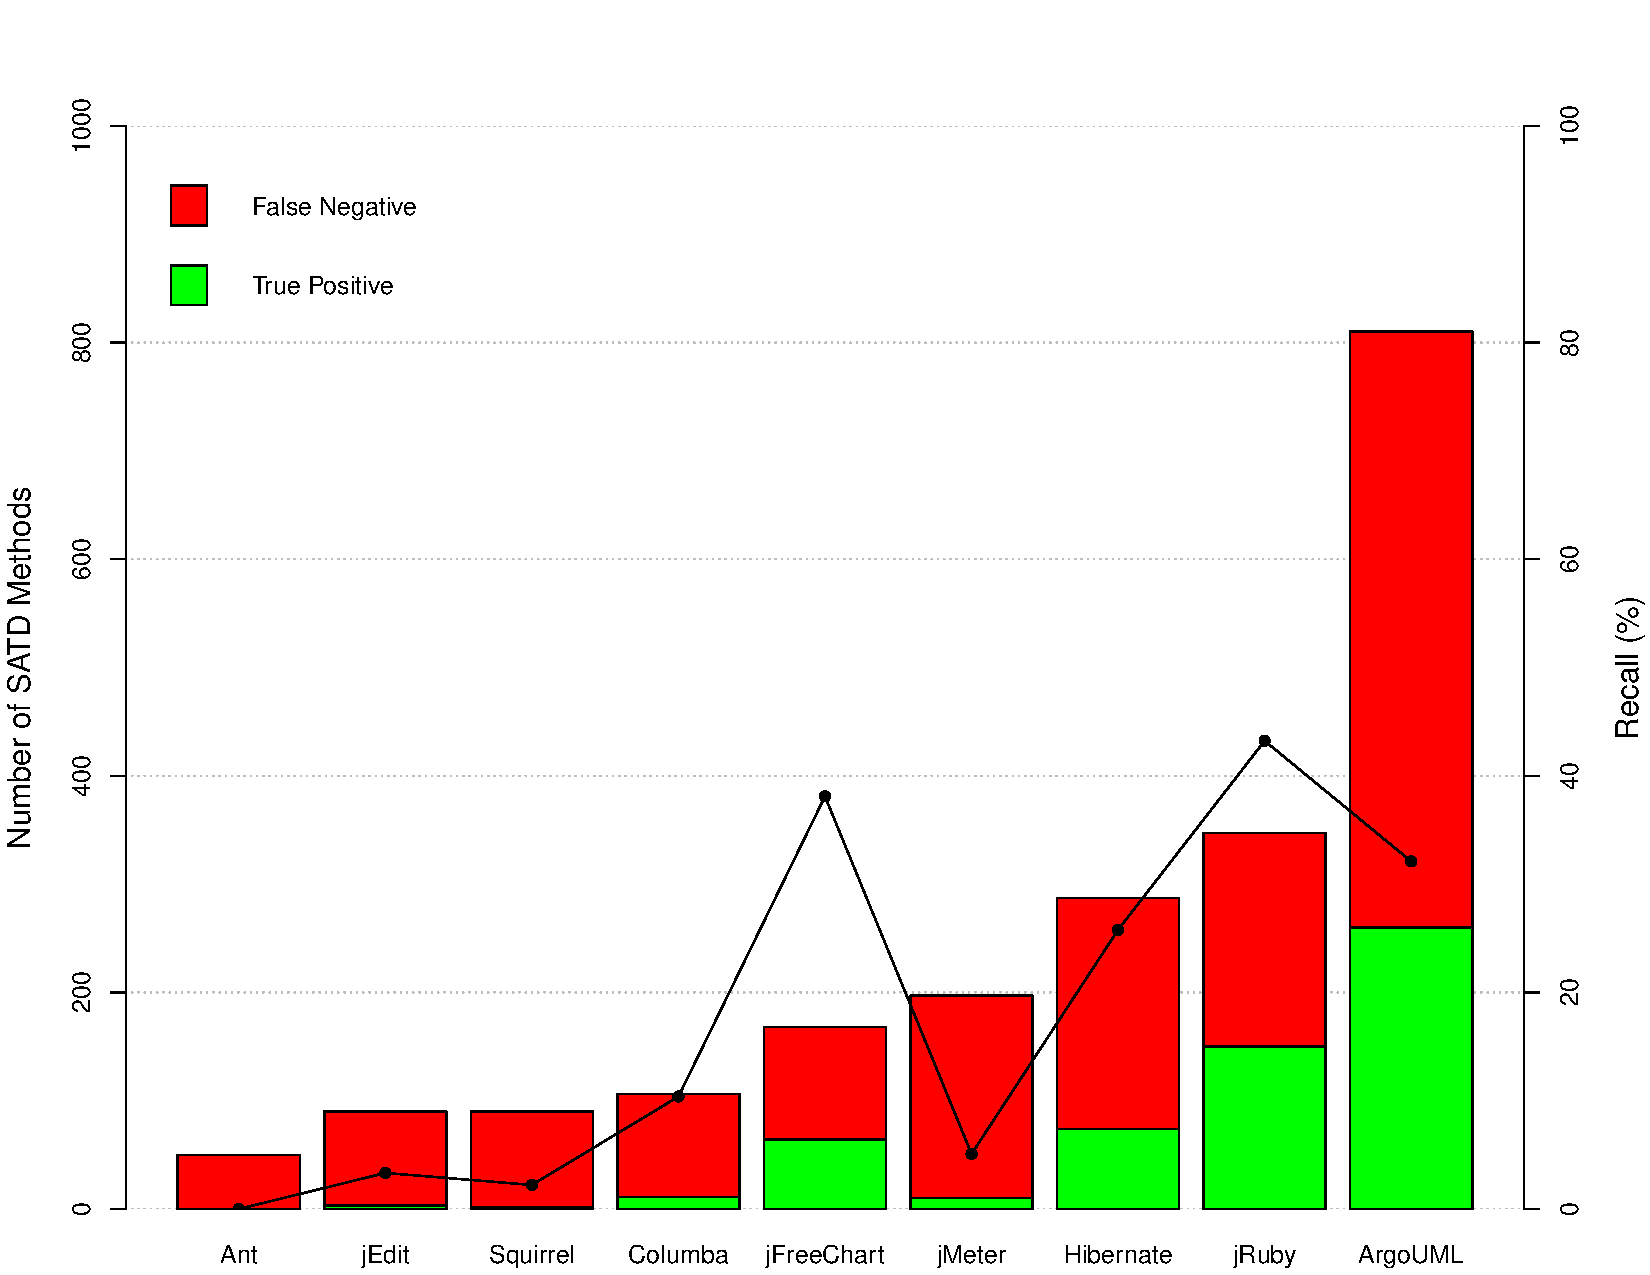
\includegraphics[scale=0.5]{figs/no-comments-pred.pdf}
	\caption{Methods without comments predictions.}
	\label{fig:no-comments-pred}
	\vspace{-4mm}
\end{figure}

\textsc{Ant} is still the system where the CNN performs the worst (precision $0\%$, recall $0\%$ and $F_1$ $0\%$), in line with every other experiment we performed so far. \textsc{jEdit}, \textsc{jMeter} and \textsc{Squirrel} are also performing pretty poorly. We observe that \textsc{jMeter} is not performing as well as it should, considering the decent amount of SATD methods it contains. It was performing well in the previous two configurations, but we could already see that it was not following the trend where performance was better in presence of more positive examples. We can visualize this observation in Figure \ref{fig:no-comments-pred}.

Differently from the other configurations, \textsc{jRuby} obtains the best performance values (precision 75.00\%, recall 43.23\% and $F_1$ 54.84\%). It contains the second most number of SATD methods, which could explain why it obtains the best results. \textsc{jFreeChart} still performs well with a precision of 75.29\% and a recall of 38.10\%., as well as \textsc{ArgoUML} with a precision of 78.31\% and a recall of 32.10\%.

\begin{table}[t]
	\caption{Within-project prediction: results of CNN for each system using source code partially with comments}
	\label{tab:partialcomments}
	\centering\tiny
	\resizebox{\linewidth}{!}{
		
		\begin{tabular}{lrrrr}
			%\hline
			\multicolumn{5}{c}{ \textbf{Source Code Partially With Comments}}\\
			\hline
			\textbf{System} & \textbf{Pr} & \textbf{Rc }&\textbf{F$_{1}$} &\textbf{Acc}\\
			\hline
			Ant & 60.00 & 6.00 & 10.91 & 99.59\\
			ArgoUML &66.97& 27.04& 38.52& 91.81\\
			Columba & 75.00 & 8.49 & 15.25 & 98.83\\
			Hibernate & 52.44 & 14.98 & 23.31 & 97.11\\
			jEdit & 0 & 0 & 0 & 98.29\\
			jFreeChart & 82.14 & 27.38 & 41.07 & 97.69\\
			jMeter & 32.14 & 4.57 & 8.00 & 97.89\\
			jRuby & 72.55 & 31.99 & 44.40 & 96.47\\
			Squirrel & 75.00 & 3.33 & 6.38 & 99.04\\
			\textbf{Total} & \textbf{66.22} & \textbf{20.65} & \textbf{31.49} & \textbf{97.49}\\
			\hline
		\end{tabular}
	}
	\vspace{-3mm}
\end{table}

As for other systems, performance metrics all decreased compared to the last two datasets, especially the recall. If we compare the total averages with the dataset with comments, the precision decreases by $- 15.89\%$, recall by $-47.74$ and $F_1$ by $-40.56\%$. Compared to within project predictions of TEDIOUS, the precision is generally better but the recall rate is worst. It is difficult, with the available information, to determine which machine learner performs better between TEDIOUS and the CNN using source code without comments. However, it is safe to say that TEDIOUS is better performance-wise, with TEDIOUS providing better recall and $F_1$ score and the CNN better precision.

\begin{figure}[t]
	\centering
	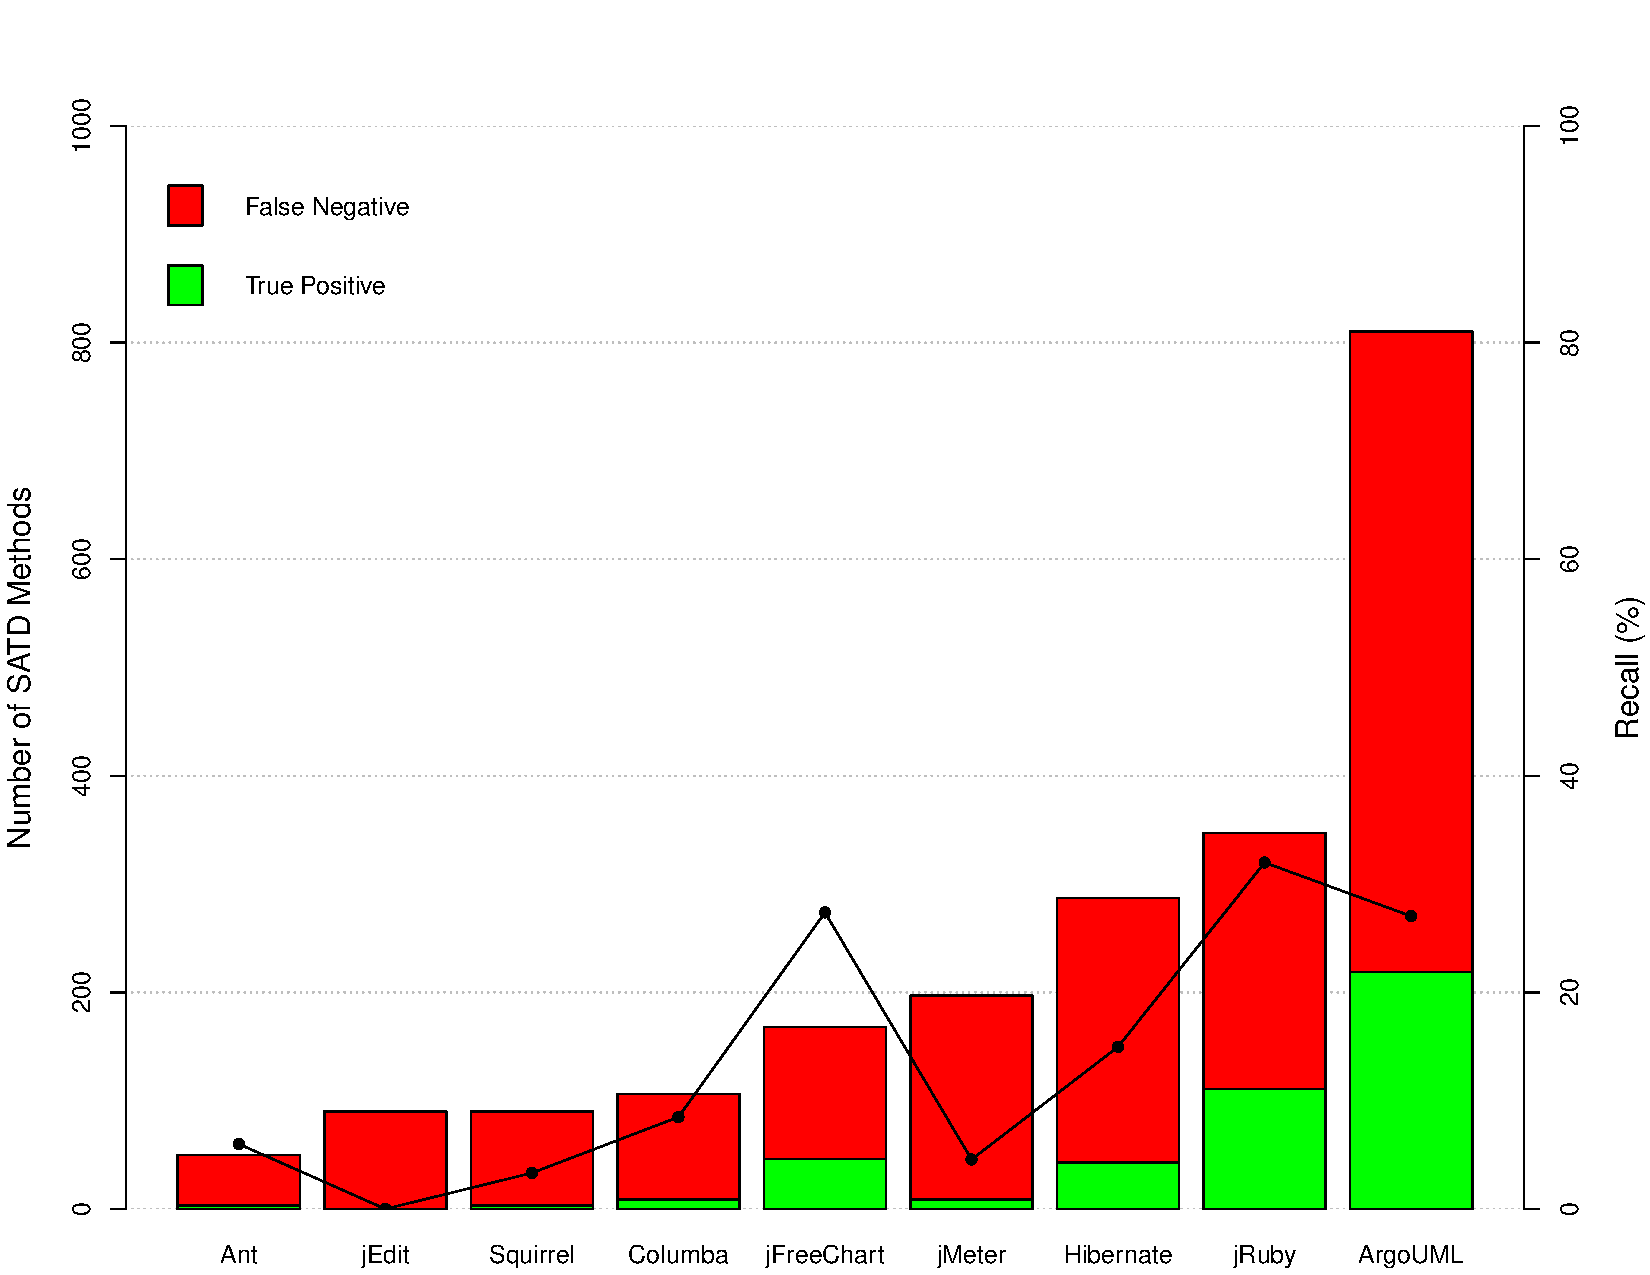
\includegraphics[scale=0.5]{figs/no-satd-pred.pdf}
	\caption{Methods and comments without SATD-comments predictions.}
	\label{fig:no-satd-pred}
	\vspace{-4mm}
\end{figure}

Overall, it is obvious that removing comments from the dataset impacts the performance of our CNN at all levels. It is clear that they represent an important piece of information for the machine learner to train on and should be kept in the dataset. We also notice that not only the number of technical debts in a system is important to obtain good performance, but the nature of technical debts and the content of the source code as well. When removing comments, we observed that the performance rank of systems differed from the previous two configurations, despite having the same number of SATD-methods in each dataset. Knowing the importance of comments, one more experiment was conducted to better understand this observation.

% \Desktop\stats-baseline-with-no-comments.csv
% dans \yes-and-no pour le data
% dans \run-all.v2.sh pour le process

\subsection{Source Code Partially With Comments}

%1.5 pages

So far, the best results were obtained with a dataset consisting of source code with comments. When removing all comments, we observed a significant loss in recall and precision. We now want to test an intermediate dataset where we keep all comments except the SATD comments manually analyzed by \citet{maldonado17}. The main reason behind the generation of this new dataset is to quantify the impact of these specific comments on the prediction performance and to know if they act as a self-prophecy. In other terms, we want to know how well our convolutional neural network can predict technical debts in methods if we remove comments self-admitting them. Table \ref{tab:partialcomments} reports the performance results for each system using a 10-fold cross validation and source code partially with comments.

% \Desktop\stats-baseline-no-manually-tagged-comments.csv
% dans \yes-and-no pour le data
% dans \run-all.v2.sh pour le process

Overall, systems perform pretty poorly, with \textsc{Ant}, \textsc{jEdit}, \textsc{jMeter} and \textsc{Squirrel} still being the most problematic ones. \textsc{jEdit} have no SATD methods being correctly predicted and the three others have at most a recall of 6.00\%. If we analyze the other projects, the precision varies between $[52.44\%-82.14\%]$, the recall between $[8.49\%-31.99\%]$ and the $F_1$ score between $[15.25\%-44.40\%]$. In other terms, the CNN is able to predict only one out of five technical debts in a system, with a decent precision. 

% \hl{All systems perform decently well and previously problematic ones, such as \textsc{Ant} and \textsc{jEdit}, are not outsiders anymore. The precision varies between $[87.23\%-100.00\%]$, the recall between $[39.09\%-68.78\%]$ and the $F_1$ score between $[56.21\%-80.52\%]$. In other terms, the CNN is able to predict at least half of the technical debts in a system with a very high precision. 

Like the dataset with all comments, results still seem dependent on the system but are weaker than previously. Compared to the dataset without comments, there is no clear trend in which configuration is better than the other. Some systems improve and others don't. However, a slight edge could be given to the dataset without comment since the recall is better and the individual performance of systems is also mostly better. In fact, source code partially with comments positions itself right next to source code without comments and below source code with comments, with a precision of 66.22\%, recall of 20.65\% and $F_1$ score of 31.49\%. Compared to TEDIOUS, our CNN without SATD comments is not considered an improvement.

% Compared to the dataset with all comments where results seemed somewhat dependent on the system, this one provides more balanced but weaker overall results. However, there is a net improvement compared to the dataset without comments. In fact, source code partially with comments positions itself right between the previous two datasets with a precision of 94.84\%, recall of 58.83\% and $F_1$ score of 72.61\%. Compared to TEDIOUS, our CNN with source code partially with comments is also an improvement.

In fact, with this experiment, we notice that SATD-related comments have an important impact on the prediction performance. The amount of comments removed in this dataset is very small compared to the total, however, the impact on performance is important, both on precision and recall. It seems like comments, especially SATD-related, are important features for our machine learner to train on. 

We observe this fact by the way each system positions itself compared to others, some will benefit from keeping SATD-related comments and others will not. Also, results without and partially with comments are really similar. Even if we add a large amount of information in the form of comments (\textit{without} compared to \textit{partially with comments}), the performance is not improving. A small amount of SATD-related comments have a larger impact on performance metrics than a large number of unrelated comments (\textit{partially} compared to \textit{with comments}). In addition, performance metrics globally decrease when removing comments.

% \hl{We observe that SATD comments have an important impact on the prediction performance. The amount of comments removed is very small compared to the total, however, the impact on performance is not negligible, mostly on recall. It seems like comments, especially SATD-related, are important features for our machine learner to train on. We observe this fact by the way each systems position themselves compared to others, some will benefit from keeping SATD-related comments and others will not. In addition, performance metrics globally decrease when removing comments.}


















